\par \textbf{Introduction}
\newline
\vspace{0.125in}
\par Most Calculus textbooks are long and boring with seemingly endless and sometimes meaningless examples. This text is an attempt to solve that problem with comprehensive yet concise explanations for all of the topics covered in the AP Calculus AB exam for the 2016-17 school year. As the text does not provide many examples, most of the topics are presented in an abstract way and I strongly recommend this text be supplementary to another textbook.\\\par All trigonometry is in radians.\\\par This textbook will have example problems throughout but exercises will be used as more of a checkpoint for the reader rather than homework.\\\par I left the margins at the default \LaTeX\, width so the reader may make notes and mark up the text. Take advantage of it!\\\par If you have any comments or suggestions about the textbook or math in general, feel free to email me. You can reach me at noah.stockwell@edgewoodhs.org.
\vfill
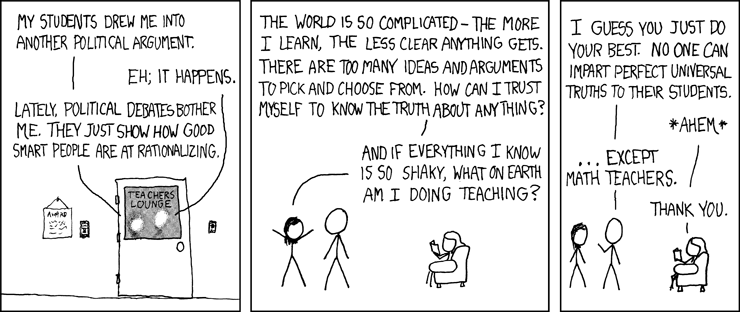
\includegraphics[width=\textwidth]{teachers.png}
\vfill
